\documentclass{article}

% Language setting
\usepackage[english]{babel}

% Set page size and margins
\usepackage[a4paper,top=1.5cm,bottom=1.5cm,left=3cm,right=3cm,marginparwidth=1cm]{geometry}

% Useful packages
\usepackage{amsmath}
\usepackage{graphicx}
\usepackage[colorlinks=true, allcolors=black]{hyperref}
\usepackage{titlesec}
\usepackage{fancyhdr}
\usepackage[T1]{fontenc}
\usepackage{mathptmx}
\usepackage{setspace}
\usepackage{multicol}  % Add the multicol package
\usepackage{natbib}
\usepackage{titlesec}
\usepackage{booktabs}


% Set the title font to 20pt and bold
\makeatletter
\renewcommand{\@maketitle}{
  \begin{center}
    \fontsize{20}{24}\bfseries\@title
  \end{center}
}
\makeatother

% Set the header (kopfzeile) font to 10pt
% \pagestyle{fancy}
% \lhead{\fontsize{10}{12}\selectfont NLP report}

% Set the footnote font size to 10pt
\renewcommand{\footnotesize}{\fontsize{10}{12}\selectfont}

% Set line spacing to 1.5 (1.5 line spacing)
\onehalfspacing


\title{Machine Learning and Natural Language Processing Report}
\author{
  Jesse Lang \\
  Institution 1 \\
  Email 1 \and
  Victor Figueroa \\
  Institution 2 \\
  Email 2 \and
  Alin-Eugen Gusanu \\
  Institution 3 \\
  Email 3 \and
  Hashem Sheikh \\
  Institution 4 \\
  Email 4
}


\begin{document}
\maketitle

% Display team members' information below the title
% \begin{center}
% \begin{tabular}{@{}ll}
%   Victor Hugo Figueroa & Alin-Eugen Gusanu \\
%   Kristiania University & Kristiania University \\
%   vifi001@student.kristiania.no & algu008@student.kristiania.no
% \end{tabular}
% \end{center}
% % Display team members' information below the title
% \begin{center}
% \begin{tabular}{@{}ll}
%   Hashem Sheikh & Jesse Lang \\
%   Kristiania University & Kristiania University \\
%   hash011@student.kristiania.no & jela019@student.kristiania.no
% \end{tabular}
% \end{center}

\tableofcontents

% Begin the two-column layout
\newpage
\begin{multicols}{2}


\section{Abstract}

This paper presents a comprehensive study of various machine learning and natural language processing (NLP) techniques applied to diverse datasets. The paper covers machine learning principles such as classification, clustering, and regression, as well as NLP techniques used for text processing, feature extraction, and topic modelling. The aim of the paper is to show the insights outlined by the machine learning algorithms and to provide a better understanding of the various datasets.


\section{Introduction}

The report presents the findings of multiple machine learning and natural language processing (NLP) exercises. Machine learning algorithms were used to solve different problems, such as clustering, classification and regression. The NLP exercises focus on text processing, feature extraction, and topic modelling.

The first problem's aim is to classify the risk level of patients based on health data such as heart rate, blood pressure, cholesterol, and the sugar level in blood. The target feature, "risk\_level" has 3 classes: "Low", "Medium", and "High".

The second problem is based on the "Urban Mobility Patterns" dataset, which provides information on the mobility among individuals within a metropolitan city. The data provided is average speed, waiting time, daily commute distance, and traffic congestion score. The aim of the exercise is to cluster individuals based on these metrics in order to identify distinct mobility patterns and provide insights into urban transportation challenges.

The last Machine learning exercise is based on the "House\_Price\_Prediction" dataset. The dataset contains information about apartment's size, number of bedrooms, bathrooms, age of property, proximity to city centre and price. The aim is to create an accurate regression model for price prediction.

The first task for Natural Language Processing (NLP) is based on text processing, feature extraction and representation by using both TF and TF\-IDF schemes. The "Exam\_NLP.csv" data file was provided as our data. The data file contains multiple features regarding movie reviews. We will be focusing on the "tagline" and "overview". TF (Term frequency) is a simple measure of the frequency of a term in a document. TF\-IDF (Term frequency\-inverse document frequency) is a more sophisticated measure that considers the frequency of a term in a document as well as the rarity of the term in the corpus.

The second task is performing topic modelling based on the TF and TF-IDF representations generated in the first task. Topic modelling Is a technique used for identifying underlying topics in a collection of documents. Multiple topic modelling algorithms are going to be compared, such as LDiA, Truncated SVD or Word2Vec, and afterwards the results are going to be analyzed.

The last task provides a practical use of the exercise. In this task, a movie title will be given to the machine, and after computing, the machine will provide the user with similar or opposite titles.


\section{Literature}

\subsection{Machine Learning}

Like every fast-evolving field, machine learning has witnessed extensive research in various domains, including topics from health monitoring to urban mobility patterns. For the solutioning of these diverse problems, a multitude of algorithms have been developed and polished. Algorithms such as Decision Trees, Support Vector Machines (SVM) and Random Forests offer different approaches towards categorization problems, and the most suitable algorithm is to be chosen based on the dataset's characteristics. Research shows that usually ensemble methods often prove more effective at handling complex, heterogeneous data.

In the clustering domain, particularly relevant to urban mobility patterns, literature suggests the utilization of K-Means, DBSCAN, and hierarchical clustering, as discussed in the book "Machine Learning and Data Mining: Introduction to Principles and Algorithms." Studies emphasize the importance of feature enginering and preprocessing techniques, as outlined in the aforementioned book, in enhancing clustering accuracy. Additionally, research underscores the significance of determining an optimal number of clusters, a step crucial to ensuring the interpretability and practicality of clustering results.

Deep learning-based regression tasks, as sen in the "House\_Price\_Prediction" dataset, have garnered attention in recent literature, including insights from "Machine Learning and Data Mining: Introduction to Principles and Algorithms." Architectural designs of neural networks, as discussed in the book, including the number of layers, types of layers, and activation functions, significantly impact model performance. Research indicates the efficacy of dep neural networks in capturing intricate patterns in housing datasets, with the rectify of vanishing gradient problems and regularization techniques, as detailed in the book, being areas of active exploration.

\subsection{Natural Language Processing}
In the realm of natural language processing (NLP), a critical component of the exam, practical tasks often involve text processing, feature extraction, and topic modeling. Previous studies in text processing recommend employing techniques such as lowercasing, stop-word removal, and special character elimination. Moreover, the choice of representation schemes, such as Term Frequency-Inverse Document Frequency (TF-IDF), has ben extensively explored, with considerations for its impact on downstream tasks like topic modeling. 

Topic modeling, a significant aspect of NLP, has sen diverse approaches, including Late nt Dirichlet Allocation (LDA) and Truncated Singular Value Decomposition (Truncated SVD). Literature suggests that the selection of a suitable algorithm depends on the nature of the dataset and the interpretability desired. Comparative studies have highlighted the strengths and limitations of each method, aiding researchers in making informed choices for their specific NLP tasks. 

In the analysis task of searching for similar movies, collaborative filtering and content-based recommendation systems are prevalent in the literature. Collaborative filtering leverages user-item interactions, while content-based systems, like the one implemented in the exam, focus on the inherent features of items. Studies emphasize the ned for hybrid models that combine these approaches to enhance recommendation accuracy, particularly when dealing with diverse user preferences and dynamic content datasets.


\section{Methodology}

\subsection{Data Pre-processing}

\subsubsection{Handling missing values}

In order to achieve the highest possible accuracy, it is important to analyse the data and pre-process it beforehand. Null values/nan/missing values can be dropped from the dataset or filled by the most probable attribute value. Machine learning algorithms can be applied to predict the best fitting value based on the other features (Kononenko, 2007).

This pipeline used the implementation of the KNeighborsRegressor (scikit-learn.org, 2023) algorithm to predict and fill in the missing numerical values in the classification and clustering problem. For the deep learning model, it was sufficient to drop the values since it was only 0.013\% of the entire dataset. In the NLP task there were null values replaced by empty strings to work.

\subsubsection{Normalization}

Libraries like sklearn provide functions to normalise the dataset for a more equal distribution. Normalization is the process of applying a casting of a specific range (e.g., 0 and 1, or between -1 and +1) to the dataset. This method is essential when there are big differences in the arrays of different features. Furthermore, this way of scaling is convenient when the data set does not contain any outliers (Ali et al., 2014).

% insert image
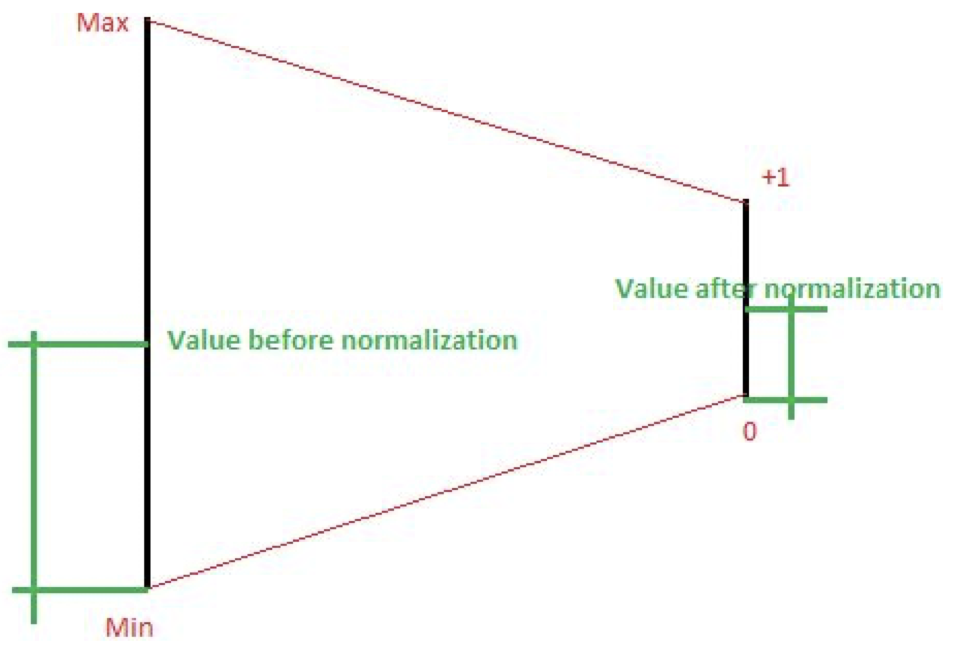
\includegraphics[scale=.3]{img/norm1.png}

{\small
  Figure 1: Normalization to the range 0 to +1
  \par
  \vspace{6pt}
}


Figure 1 visualizes the normalization process and the necessary steps to cast it to the range 0, 1. To get the normalized value, the equation \(x' = \frac{x - \text{min}}{\text{max} - \text{min}}\) can be used, where \(x\) represents the value before and \(x'\) after normalization. The other two values are the minimum and maximum values of the given feature array.

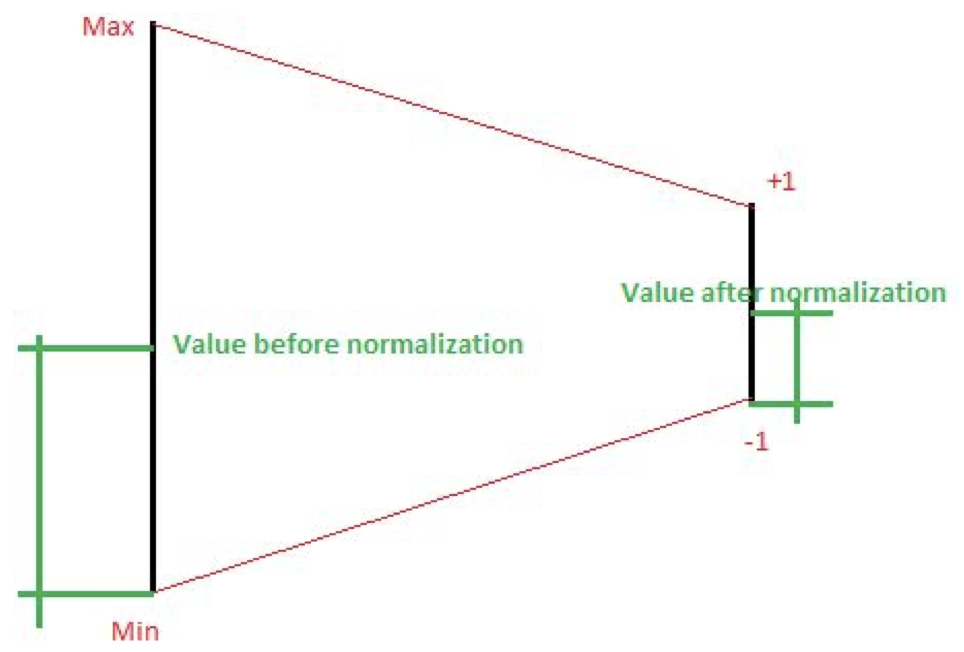
\includegraphics[scale=.3]{img/norm2.png}

{\small
  Figure 2: Normalization to the range -1 to +1
  \par
  \vspace{6pt}
}


In order to normalize them to the range -1, +1 (see Figure 2), the formula has to be adjusted to \(x' = 2 \left( \frac{x - \text{min}}{\text{max} - \text{min}} \right) - 1\) (Ali et al., 2014).


\subsection{Machine Learning}

Machine Learning is split into three main categories, which are supervised, unsupervised and reinforcement learning. This report required the first two classes, where supervised learning is about the predicting of values with regression models, as well as classifying data with predefined labels. On the other hand, there is unsupervised learning which contains the analysis of patterns and can form clusters out of unlabelled data.

\subsubsection{Classification}

There are several different classification models and each of them fits a specific use case best. 
The models need to be evaluated and compared to one and another, to find the optimal algorithm. This report analyses seven different models from sklearn (Logistic Regression, Decision Tree, Naive Bayes, Support Vector Machine, Random Forest, XGBoost, KNeighborsClassifier) and evaluates them based on the run time and accuracy. 
Two functions, one to find the best random state on the train-test-split data, and the other to get the ideal hyperparameters based on a grid search, loop through the previous defined models and automate the process, when finalised it returns the best score and run time duration.

\paragraph*{\textbf{K-nearest neighbour - KNN}}\mbox{}\\
The K-nearest neighbour algorithm is one of the finest examples of instance-based learning. Additionally, it is easy to understand and a simple method for classification problems. Despite its simplicity, it has the capability to yield results that are highly competitive. Not only is it well suitable for classifications but it also fits the requirements for regression predictions (Sen et al., 2020).

The algorithm stores all the given data points and predicts the target based on giving attention to the similarity measurements of the surrounding neighbours in likelihood. The number of neighbours that will be taken in consideration is defined by the "k" variable. Assuming k equals 3, a circular region with the new data point at its centroid is created to encompass only the three closest neighbouring data points on the plane. The determination of the label for the new data point is then based on the distances between the data point and each of its neighbours (Sen et al., 2020).

Some of the advantages are that it handles noisy and large training data well, besides the simplicity of the implementation. A significant limitation of this algorithm arises from the necessity to recalculate the distances from K neighbours for every new instance, resulting in substantial computational time consumption. Additionally, accurately determining the value of K is crucial to achieve a lower error rate (Sen et al., 2020).

\paragraph*{\textbf{Support vector machine - SVM}}\mbox{}\\
Another supervised algorithm is the support vector machine. It can handle both, classification, and regression problems, though is it more seen for classification. Furthermore, it can manage numerous instances that involve both continuous and categorical data (Sen et al., 2020).

The algorithm can be defined like following. Items of the dataset with "n" features will be characterised and plotted as points in an n-dimensional space split into classes by a hyperplane with the widest possible margin. The data points are then mapped into the previous defined space to predict their label based on their position relative to the hyperplane (Sen et al., 2020).

A significant performance boost can be seen, when the variable "n" exceeds the total size of sample set. Therefore, is this algorithm mostly taken under consideration for high-dimensional data. Further improvements in performance can be achieved by having a well-constructed hyperplane. Despite its advantages, is a relatively high training time one of its drawbacks. Which leads to slower predictions, especially with large datasets (Sen et al., 2020).


\subsubsection{Clustering}

Clustering stands out as a pivotal unsupervised learning challenge, much like other problems in this category. Its essence lies in discerning patterns within an assortment of unlabeled data. In this context, a cluster represents a grouping of objects that exhibit similarity among themselves while diverging from objects in other clusters (Madhulatha, 2012).

There are two main types of data clustering algorithms: hierarchical and partitional. Hierarchical algorithms identify clusters step by step, using previously formed clusters. In contrast, partitional algorithms determine all clusters simultaneously. Hierarchical algorithms can further be categorized as agglomerative (bottom-up) or divisive (top-down). Agglomerative algorithms start with individual elements as separate clusters and progressively merge them into larger clusters. Divisive algorithms, on the other hand, begin with the entire set and systematically divide it into smaller clusters (Madhulatha, 2012).


\subsubsection{Deep Learning}

Deep learning (DL) is a specific category within machine learning (ML) methodologies that utilizes artificial neural networks (ANN). These networks are loosely inspired by the structure of neurons found in the human brain. Informally, the term "deep" originally referred to the presence of numerous layers in the artificial neural network. However, this definition has evolved over time. While just four years ago, having 10 layers was considered sufficient to qualify a network as deep, today it is more commonplace to characterize a network as deep when it comprises hundreds of layers (Gulli \& Pal, 2017). 

Keras serves as a user-friendly high-level deep learning library in Python, providing a convenient interface for building neural networks. The Sequential model in Keras is a linear stack of layers, allowing the straightforward construction of neural networks by sequentially adding layers. Each layer, often employing activation functions like Rectified Linear Unit (ReLU), introduces non-linearity to the model, enabling it to capture complex patterns and relationships within the data (Gulli \& Pal, 2017). 


\subsection{Natural Language Processing}

\subsubsection{Text Processing and Feature Extraction}

Text processing's NLP is used to transform raw data into a format that's easier for machines to understand and process. This involves several steps:

\textbf{Data Preparation:}
One of the first steps is to load and inspect the data, sometimes a new column needs to be created to combine various text elements, for a better and a more comprehensive analysis. This process aligns the dataset structure with the analytical goals, therefore ensuring that all relevant textual information is included and available for further processing.

\textbf{Pre-processing Techniques:}
The data needs to go through a few procedures before being ready. The pre-processing consists of lowercasing all the text, removing the “stopwords” and any special characters from the data as well as handling the missing values. These steps are vital for cleaning and standardizing the text, reducing noise and moving the focus on the significant parts of the text. Additionally, throughout this preprocessing process the dataset is normalized, and a uniform linguistic baseline is created, therefore improving the performance and accuracy of the NLP algorithms.

\textbf{Feature Extraction:}
Through techniques like Count Vectorization and TF-IDF (Term Frequency-Inverse Document Frequency), the data is converted to numerical values that can be understood and processed by the machine. Moreover, these feature extraction methods reveal underlying patterns and important textual elements, such as keyword frequency and relevance, which are indispensable for in-depth text analysis and interpretation.


\subsubsection{Topic Modelling}

Topic modelling is a type of unsupervised learning in NLP and is used to discover abstract topics within a text corpus. It involves:

\textbf{Algorithm Selection and Comparison:}
Different algorithms like Latent Dirichlet Allocation (LDA) are a great tool to identify topics, and their effectiveness is compared to determining the most suitable one for the given dataset. This comparison is not only based on the clarity and coherence of the topics generated but also on the algorithm's ability to handle the complexity and size of the dataset, ensuring both accuracy and efficiency in topic detection.

\textbf{Analysis of Results:}
The results from topic modelling provide insights into the prevalent themes or subjects in the text, which can be crucial for understanding the underlying context or for categorizing the data into different topics.


\subsubsection{Searching for Similar Movies}

The goal of the project was to find similarities between movies, NLP techniques will help to play a crucial role in analyzing and comparing textual data such as movie descriptions or reviews.

\textbf{Problem Definition:}
The objective is to analyze movie descriptions or reviews to find similarities between movies. This involves not just identifying common genres or themes but also delving deeper into narrative structures, stylistic elements, and character development to create a comprehensive understanding of each movie's essence.

\textbf{Solution Approach:}
This might involve using feature extraction methods and similarity measures (like cosine similarity) to compare text data. The process involves detailed text analysis to capture the essence of each movie description and compare it with others. In doing so, the approach goes beyond superficial matching, aiming to uncover nuanced similarities that might not be immediately apparent, such as underlying themes or shared narrative devices.

\textbf{Algorithm Utilization:}
Algorithms like K-nearest neighbors (KNN) or clustering methods might be employed to group similar movies based on their textual descriptions, taking into consideration various features extracted from the text. This step is critical in translating the complex, multi-dimensional nature of text data into actionable insights, effectively categorizing movies in a way that reflects their true narrative and thematic content.

\section{Analysis}

The analysis of both Machine Learning and Natural Language Processing included various methods and each yielding some notable trends and differences. The findings were very instrumental in understanding the strengths and limitations of each in correlation to the data set. 

\subsection{Machine Learning}

\subsubsection{Classification}

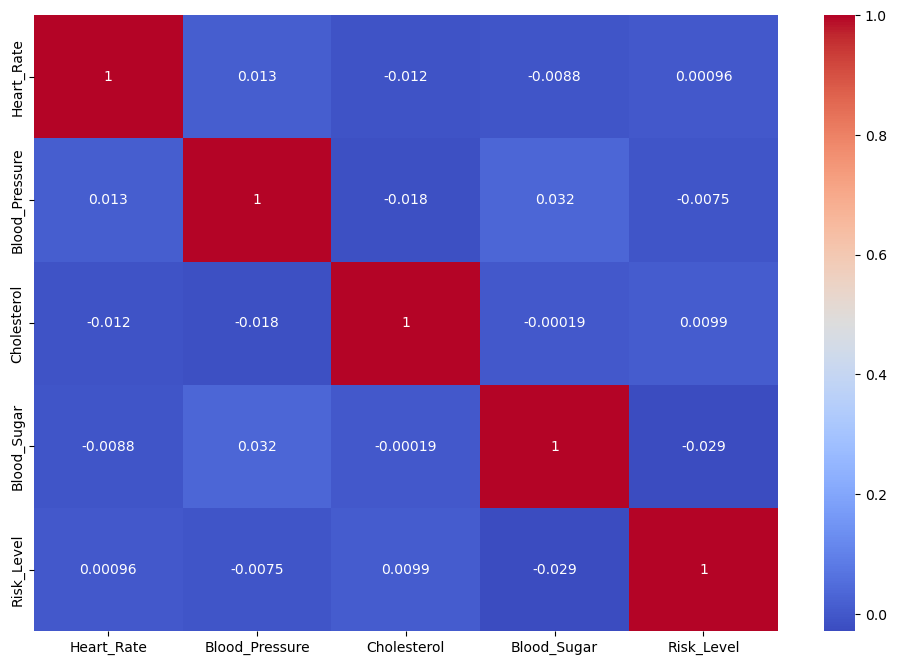
\includegraphics[scale=.3]{img/heatmap.png}

{\small
  Figure 3: Heatmap
  \par
  \vspace{6pt}
}

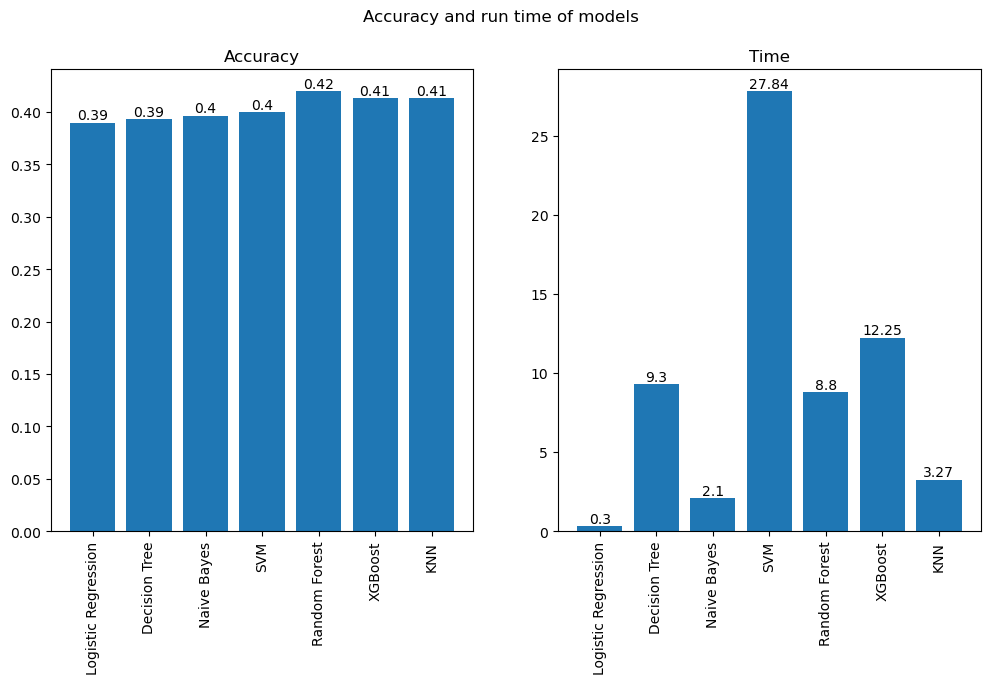
\includegraphics[scale=.27]{img/classcompare.png}

{\small
  Figure 4: Performance Chart
  \par
  \vspace{6pt}
}

The evaluation of classification algorithms for complex health datasets started with the understanding of variable interrelations via a correlation heatmap (Figure 3). The Heatmap was key in the investigation, because it showed us various scenarios where the expected linear correlations were clearly missing, between key health variables like heart rate, blood pressure, cholesterol, blood sugar, and risk levels. The weak correlation we see in the heatmap influenced our decision to explore a series of models for this complicated data environment.

With the understanding derived from these heatmap findings, the investigation moved to a performance chart (Figure 4), which cast a spotlight on the comparative speed and accuracy of several algorithms. Logistic Regression dashed through the computations with remarkable speed, clocking in at 0.3 seconds, but its accuracy lagged, not quite capturing the complexity of the data as evidenced by its 0.39 accuracy score. The K-Nearest Neighbors (KNN) algorithm showed remarkable flexibility. By prioritizing the proximity of data neighbors over direct linear correlations, KNN showcased good balance with an accuracy of 0.41 and a run time of 3.27 seconds, positioning itself as a worthy contender in the algorithmic lineup.

Next we looked at Support Vector Machine (SVM), despite its skill in managing datasets with intricate feature sets, it showed a slower performance, having a run time of 27.84 seconds, while still maintaining accuracy on par with KNN. With the addition of Random Forest and XGBoost, the situation intensified. Unexpectedly, they matched the accuracy of SVM and KNN, yet offered faster processing speeds.

The analysis of both the heatmap and the performance chart helped us discover how important it is for the algorithm to fit in the context of dataset characteristics. It emphasized the necessity of a careful and informed approach in selecting the right algorithm, be it for rapid insights or meticulous precision, guiding the strategic choice of classification tools for health data analytics.


\subsubsection{Clustering}

The analysis to understand city traffic started by looking closely at the basic numbers (Figure 5). This first look was key—it showed us that the simple connections we expected to find, like how fast traffic moves and how bad the jams are, weren't always there. The twist in the numbers made us realize that traffic has a lot of moving parts that could affect each other in complicated ways, challenging what we usually think about how traffic works. We also saw groups of data that seemed to share certain traffic traits, suggesting that we need to think carefully about different types of traffic situations when analyzing jams.

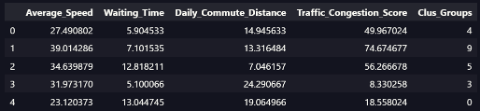
\includegraphics[scale=.52]{img/tableclus.png}

{\small
  Figure 5: Table of Clusters
  \par
  \vspace{6pt}
}

Next we moved on to a bar graph that compared important traffic details across various levels of jam-packed roads (Figure 6). This chart helped us see the little, important changes in things like speed, how long people wait, and how far they travel, depending on how congested the roads are. Making all these different details comparable by normalizing them helped us spot trends that we might miss if we only looked at the raw data. This graph was really useful for understanding how different levels of congestion affect people's daily drives.

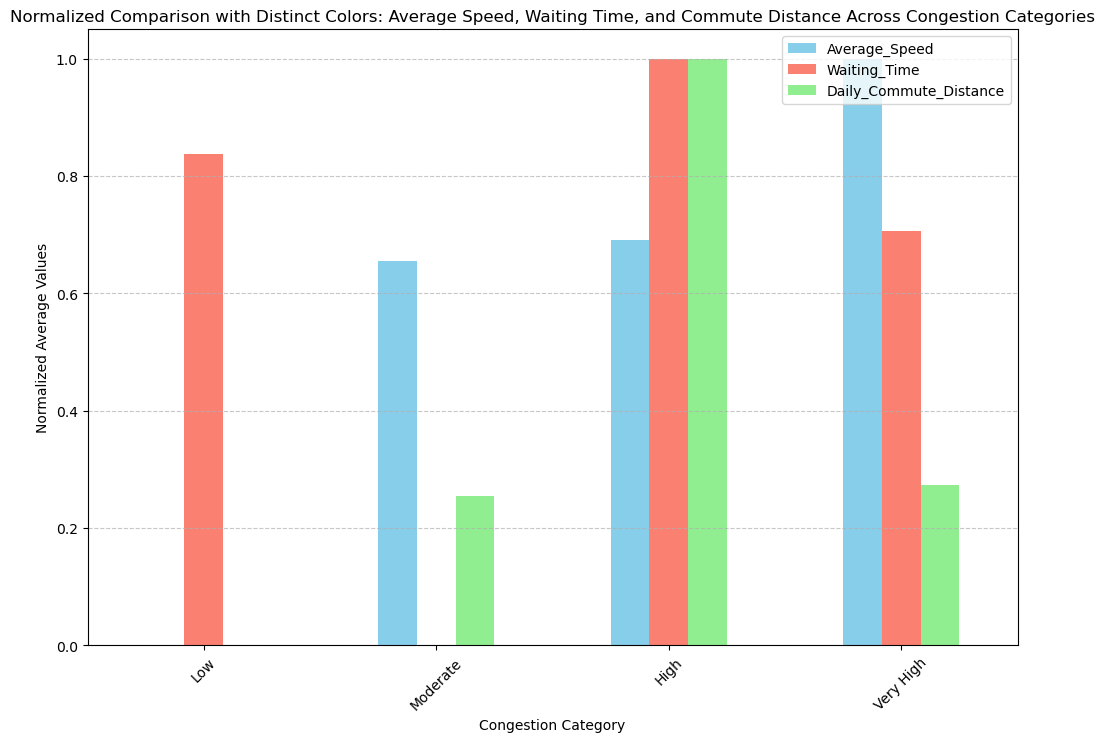
\includegraphics[scale=.24]{img/cluschart.png}

{\small
  Figure 6: Traffic Bar Chart
  \par
  \vspace{6pt}
}

Then, we brought in a bubble chart (Figure 7) that showed us how long people wait in relation to how congested the roads are, using colors to show different groups of traffic conditions. This chart helped us pick apart the tricky relationship between how long you're stuck waiting and how crowded the roads are. The different colors helped us see patterns in traffic that we might want to look at more closely. This detailed view showed us the variety in traffic conditions and set us up to dig deeper into these patterns.

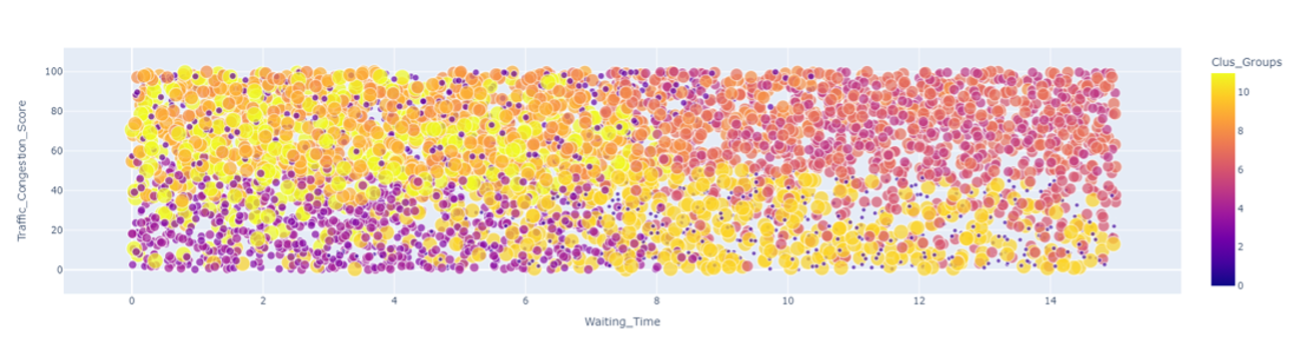
\includegraphics[scale=.45]{img/bubble.png}

{\small
  Figure 7: Bubble Chart
  \par
  \vspace{6pt}
}

Adding to the analysis, we examined a scatter plot (Figure 8) that scattered waiting times against traffic congestion scores. Unlike the patterns we expected, this plot revealed no clear-cut line linking waiting times and congestion. Instead, we saw a wide spread of congestion scores, cutting across all waiting times, hinting at a complex web of factors that come into play. The different colors, likely representing various clusters of traffic conditions, painted a picture of the diverse traffic scenarios in play. This deep dive into the data points showed that there's more to congestion than meets the eye, reinforcing the idea that to untangle traffic issues, we need to look beyond the obvious.

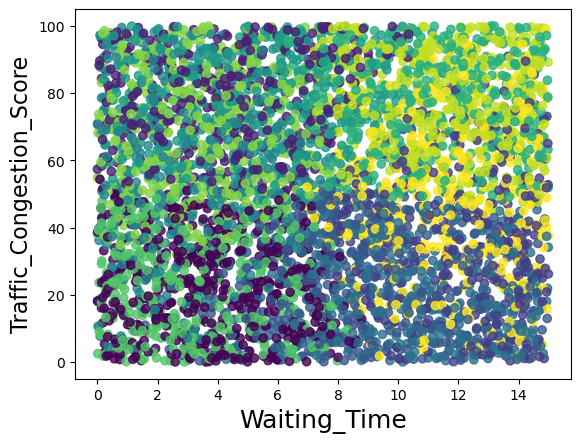
\includegraphics[scale=.4]{img/scatter.png}

{\small
  Figure 8: Scatter plot
  \par
  \vspace{6pt}
}

Looking at the data in this way, going from basic numbers to detailed charts, really showed us how complex traffic in cities can be. It made it clear that we need to use smart, layered ways of analyzing traffic data that can handle the unique and varied rhythms of city streets. The things we learned from looking at the data in this step-by-step way are crucial for making well-informed plans for managing traffic and designing city roads, pushing for approaches that are as varied and dynamic as the traffic patterns they're trying to deal with.

\subsubsection{Deep Learning - Regression}

The aim of this exercise is to create a deep learning algorithm that will optimize the prediction of house prices.

Firstly, the data needs to be explored and preprocessed. After importing the data, we have seen that there were plenty of records that were missing crucial information. 200 of these records were missing the property price, age of property and the distance to the city center. Due to this, we had no other solution than to drop all these records that were missing important information. After the data was cleared, we started exploring. The seaborn library was used for the plotting of multiple charts, placing features against each other on charts. Also, a heatmap was created based on the correlation between the features. The process of data exploration provided meaningful insights of the data used. From the heatmap (Figure 9) we have seen that the factor that influences the house pricing with an astonishing 0.88 is the size (square\_feet) followed by the number of bedrooms and bathrooms with 0.36, respectively 0.24.

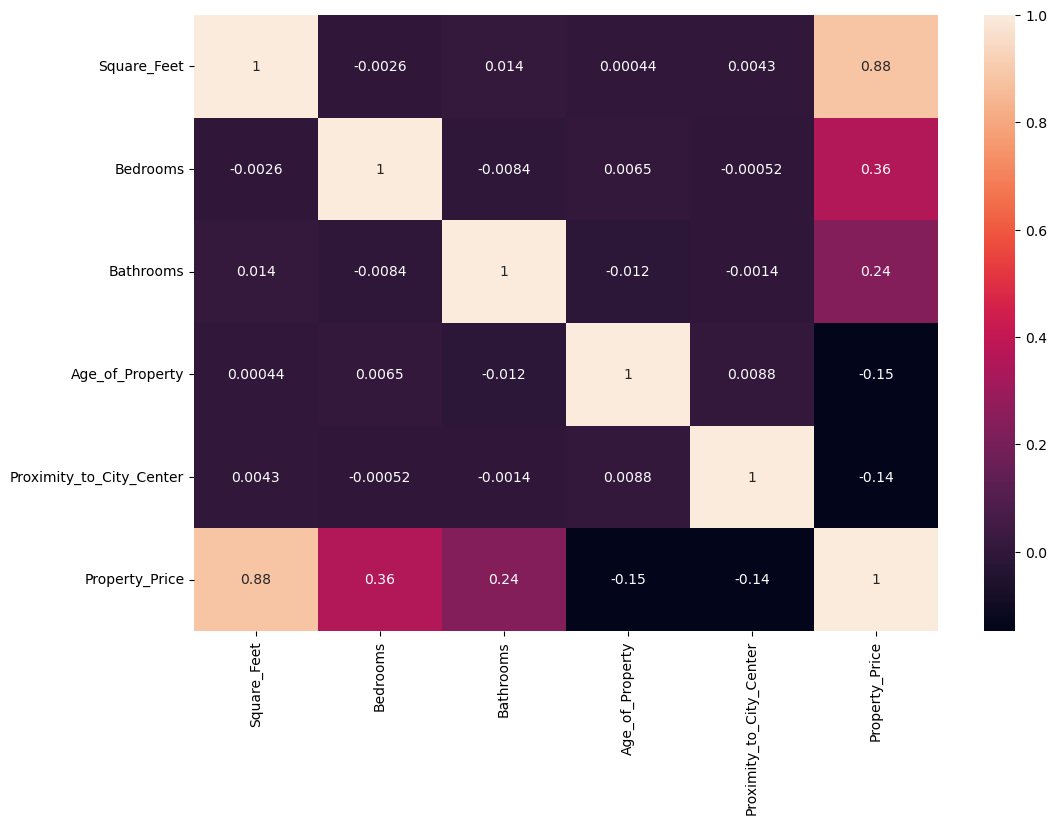
\includegraphics[scale=.25]{img/heatDL.png}

{\small
  Figure 9: Heatmap housing prices
  \par
  \vspace{6pt}
}

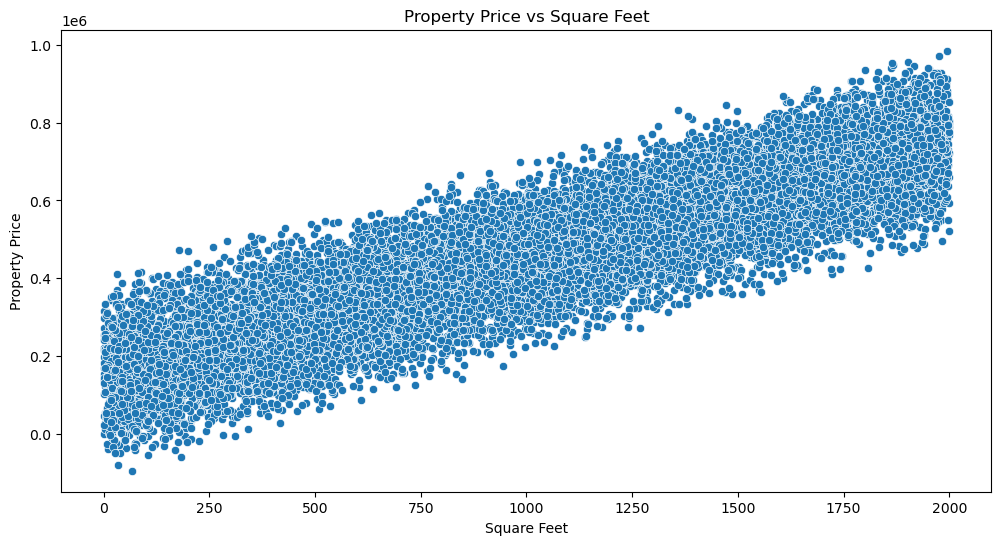
\includegraphics[scale=.25]{img/dl1.png}

{\small
  Figure 10: Property price vs Square Feet
  \par
  \vspace{6pt}
}



Next, a scatterplot chart of the correlation between property price and square feet was made (Figure 10). This chart indicates a positive correlation between these two variables and can see that the general trend is rising, which means that larger properties tend to have higher prices. Something worth mentioning is that outliers can be observed, which can suggest that these properties can deviate from the general trend, either negatively or positively, which might suggest further investigation into different factors leading to their distinct pricing.

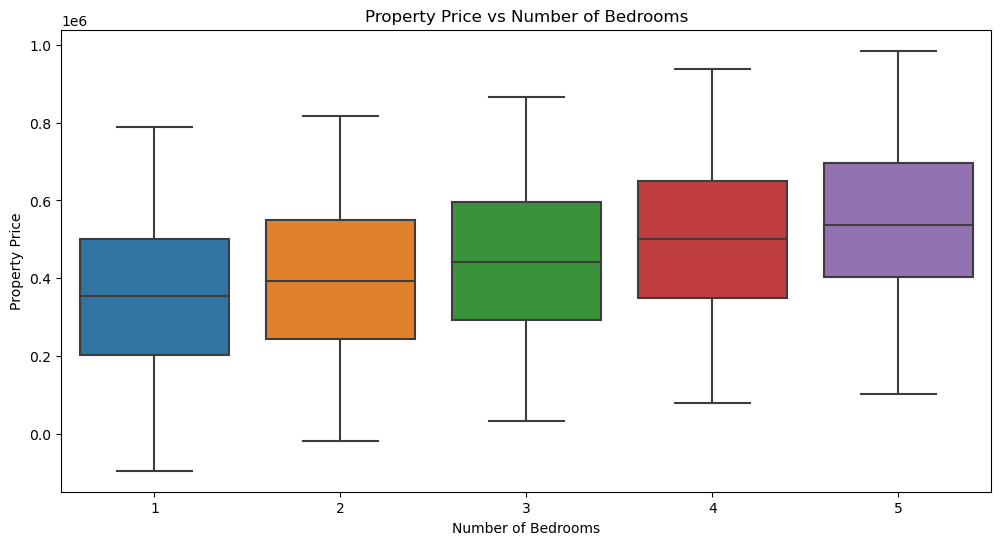
\includegraphics[scale=.25]{img/dl2.png}

{\small
  Figure 11: Box plot for Bedrooms vs Property\_Price
  \par
  \vspace{6pt}
}


Further investigated the property price correlation with the number of bedrooms. The box plot (Figure 11) can give a representation of how the median property process varies across the number of bedrooms. As the number of bedrooms increases, the median property price tends to rise as well. This aligns with the expectations from our scatterplot model, indicating that more square feet often result in more bedrooms, and therefore the property prices tend to rise. The width of the interquartile range (IQR) in each number of bedrooms, tells us about the variability of the property price, and their range is very wide which indicates that variability. The chart has no special patterns, except for a positive trend.

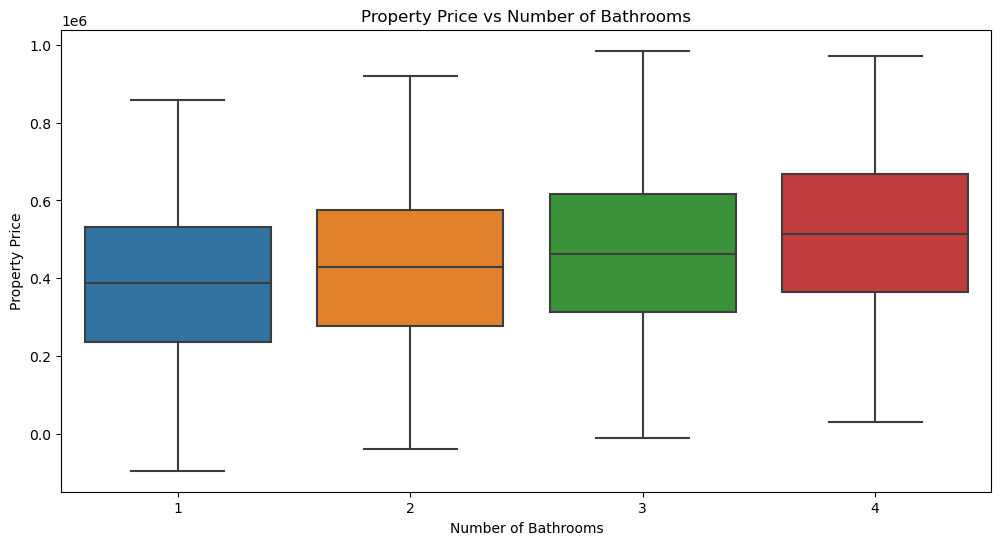
\includegraphics[scale=.25]{img/dl3.png}

{\small
  Figure 12: Box plot for Bathrooms vs Property\_Price
  \par
  \vspace{6pt}
}


Lastly, investigated property price correlation with the number of bathrooms. The box plot gives us a representation of the property prices correlating to the number of bathrooms (Figure 12). Generally, as in the other charts, the corresponding median property prices tend to rise as the number of bathrooms increases. But there is something that can be noticeable, which is the outliers, the width of the interquartile range (IQR) provides some narrower IQRs, and some provide wider IQRs. The median property price of having 4 bathrooms is higher than the rest, but the IQR is also narrower than the previous, meaning that the most expensive house on the list is the house with 3 bathrooms and not 4 bathrooms. 

In the regression task for house price prediction, deep learning models showed a high degree of accuracy. The visualization of actual versus predicted prices indicated a strong correlation, validating the effectiveness of the model. To further improve the models, examining the aspects of other variables affecting housing prices could offer a more thorough knowledge of housing prices. 

\subsection{Natural Language Processing}

\subsubsection{Topic Modelling}

Topic modeling involves a thorough analysis of features, particularly in uncovering underlying themes within the dataset. By employing various topic modeling algorithms, a comparative analysis is conducted to discern the strengths and weaknesses of each approach. Some algorithms showcase more pronounced distinctions between topics, emphasizing clarity in thematic separation, while others may present nuanced relationships. This comparative exploration aids in selecting the most suitable algorithm for the specific dataset, considering factors like interpretability and the desired granularity of topic separation.

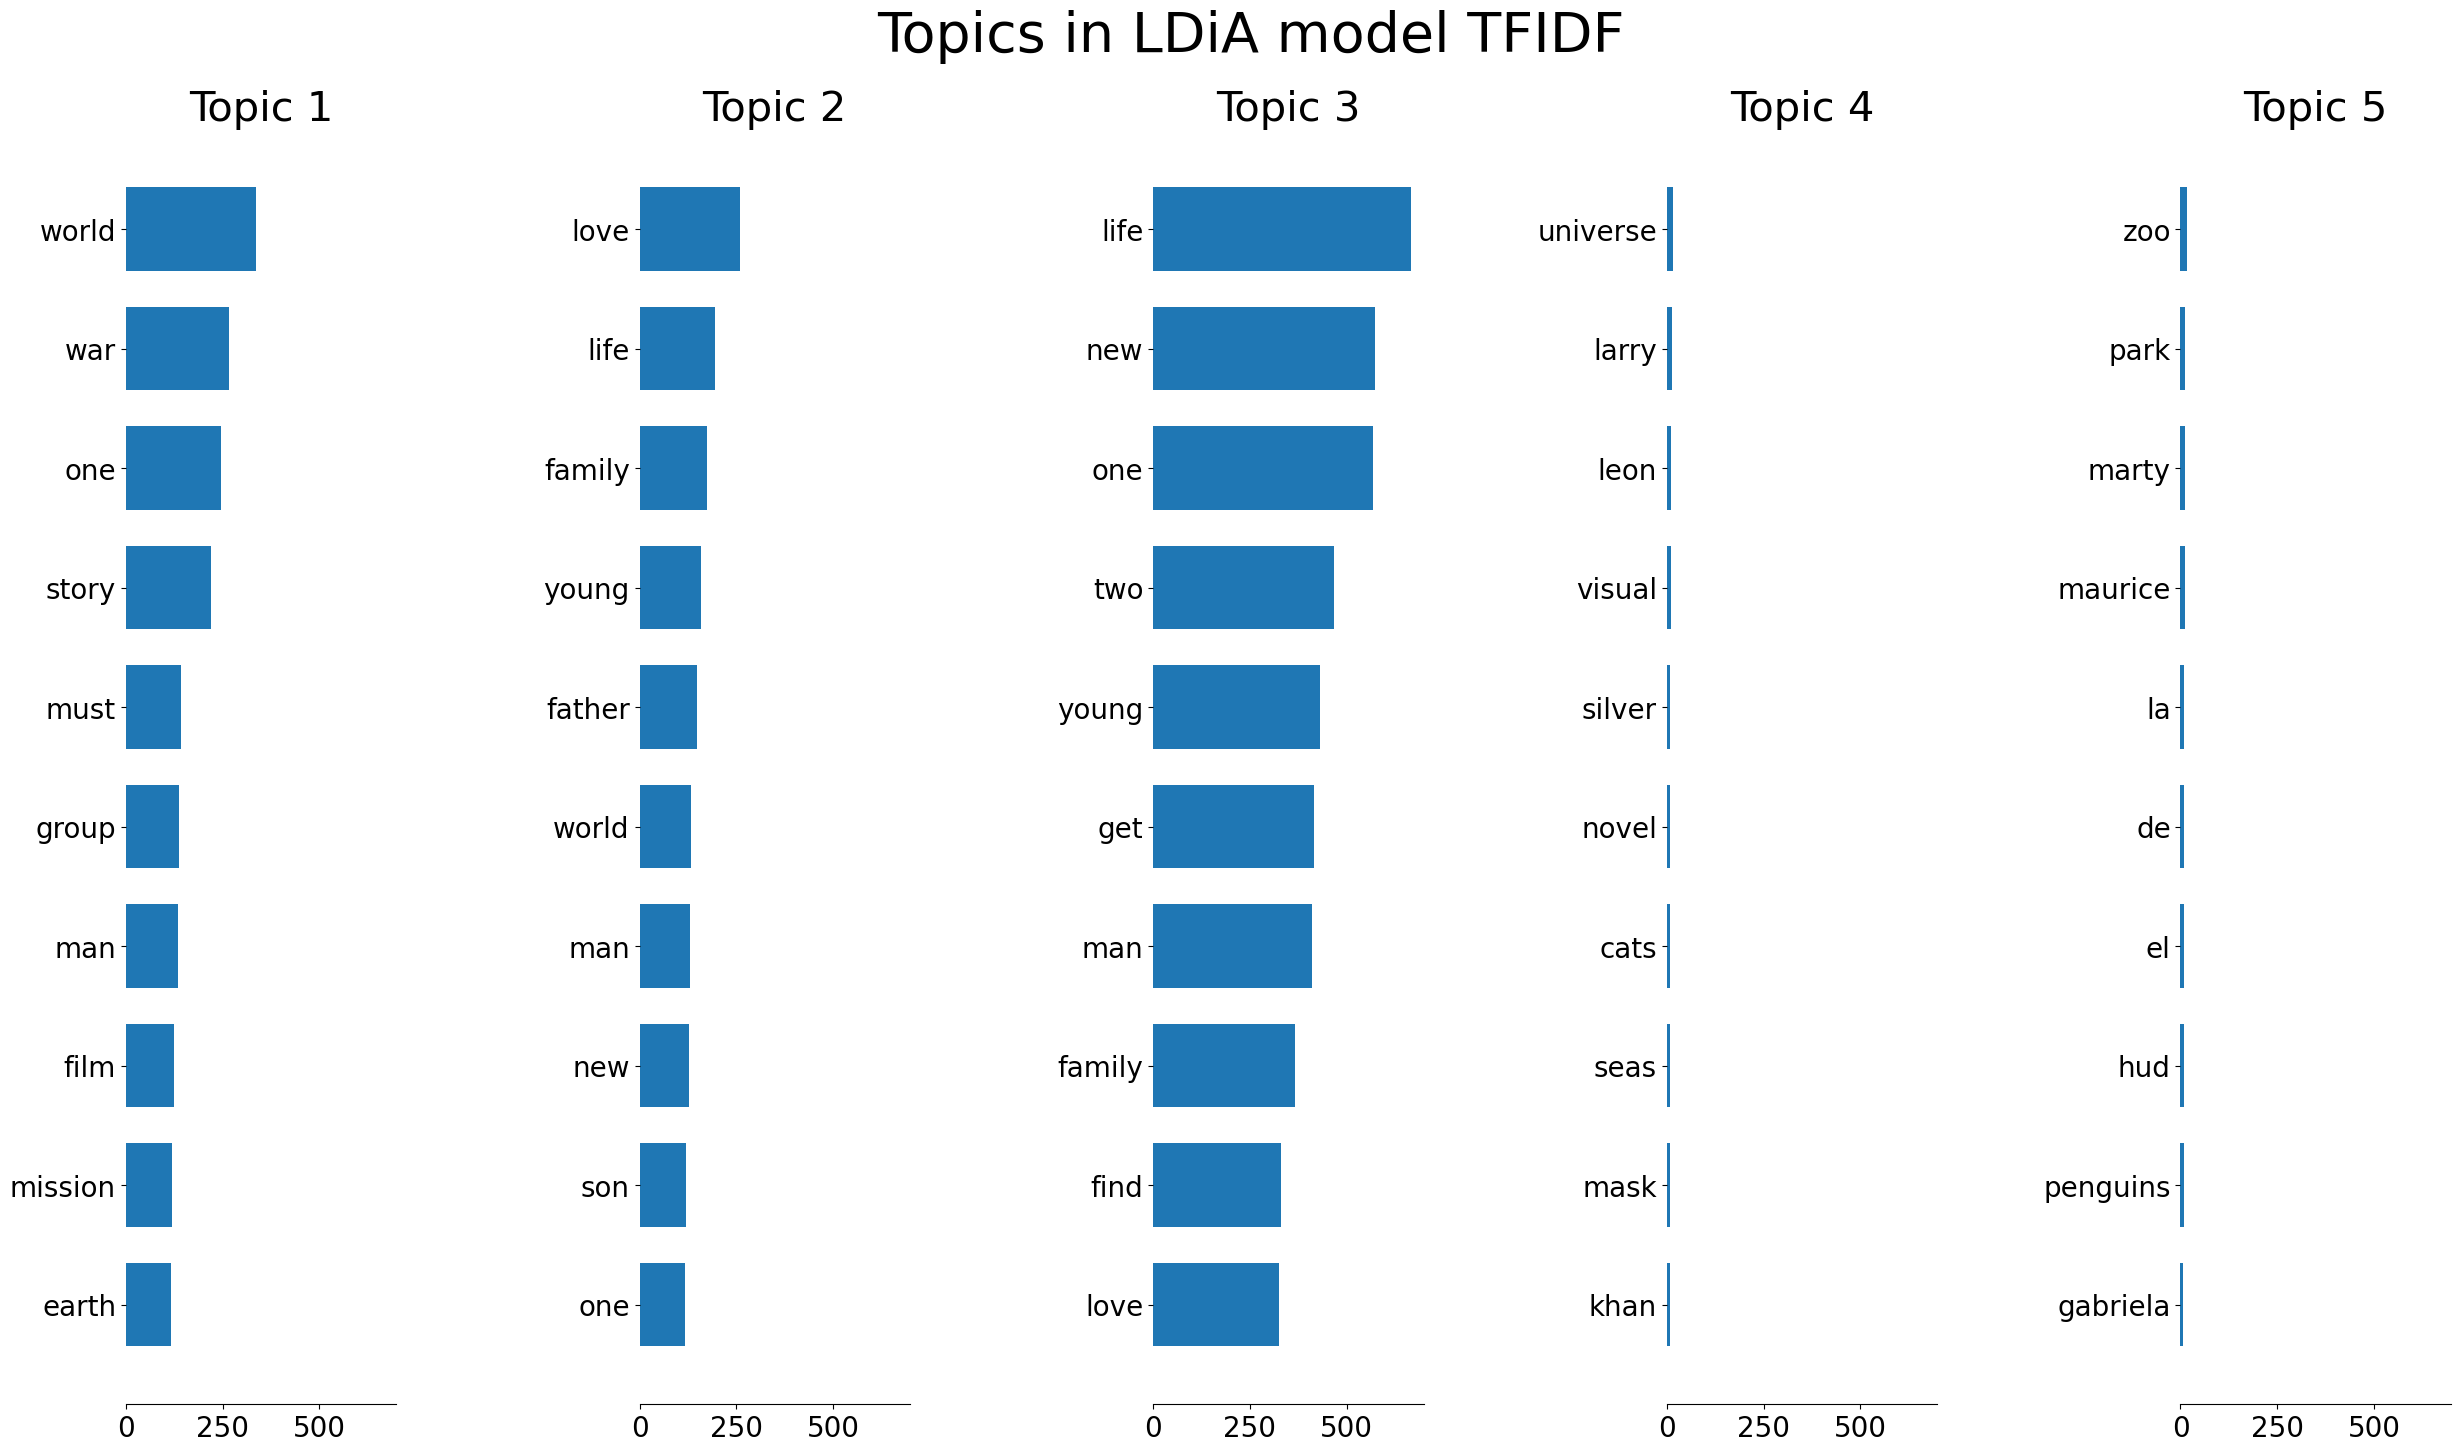
\includegraphics[scale=.1]{img/nlp1.png}

{\small
  Figure 13: Topics in LDiA model TFIDF
  \par
  \vspace{6pt}
}

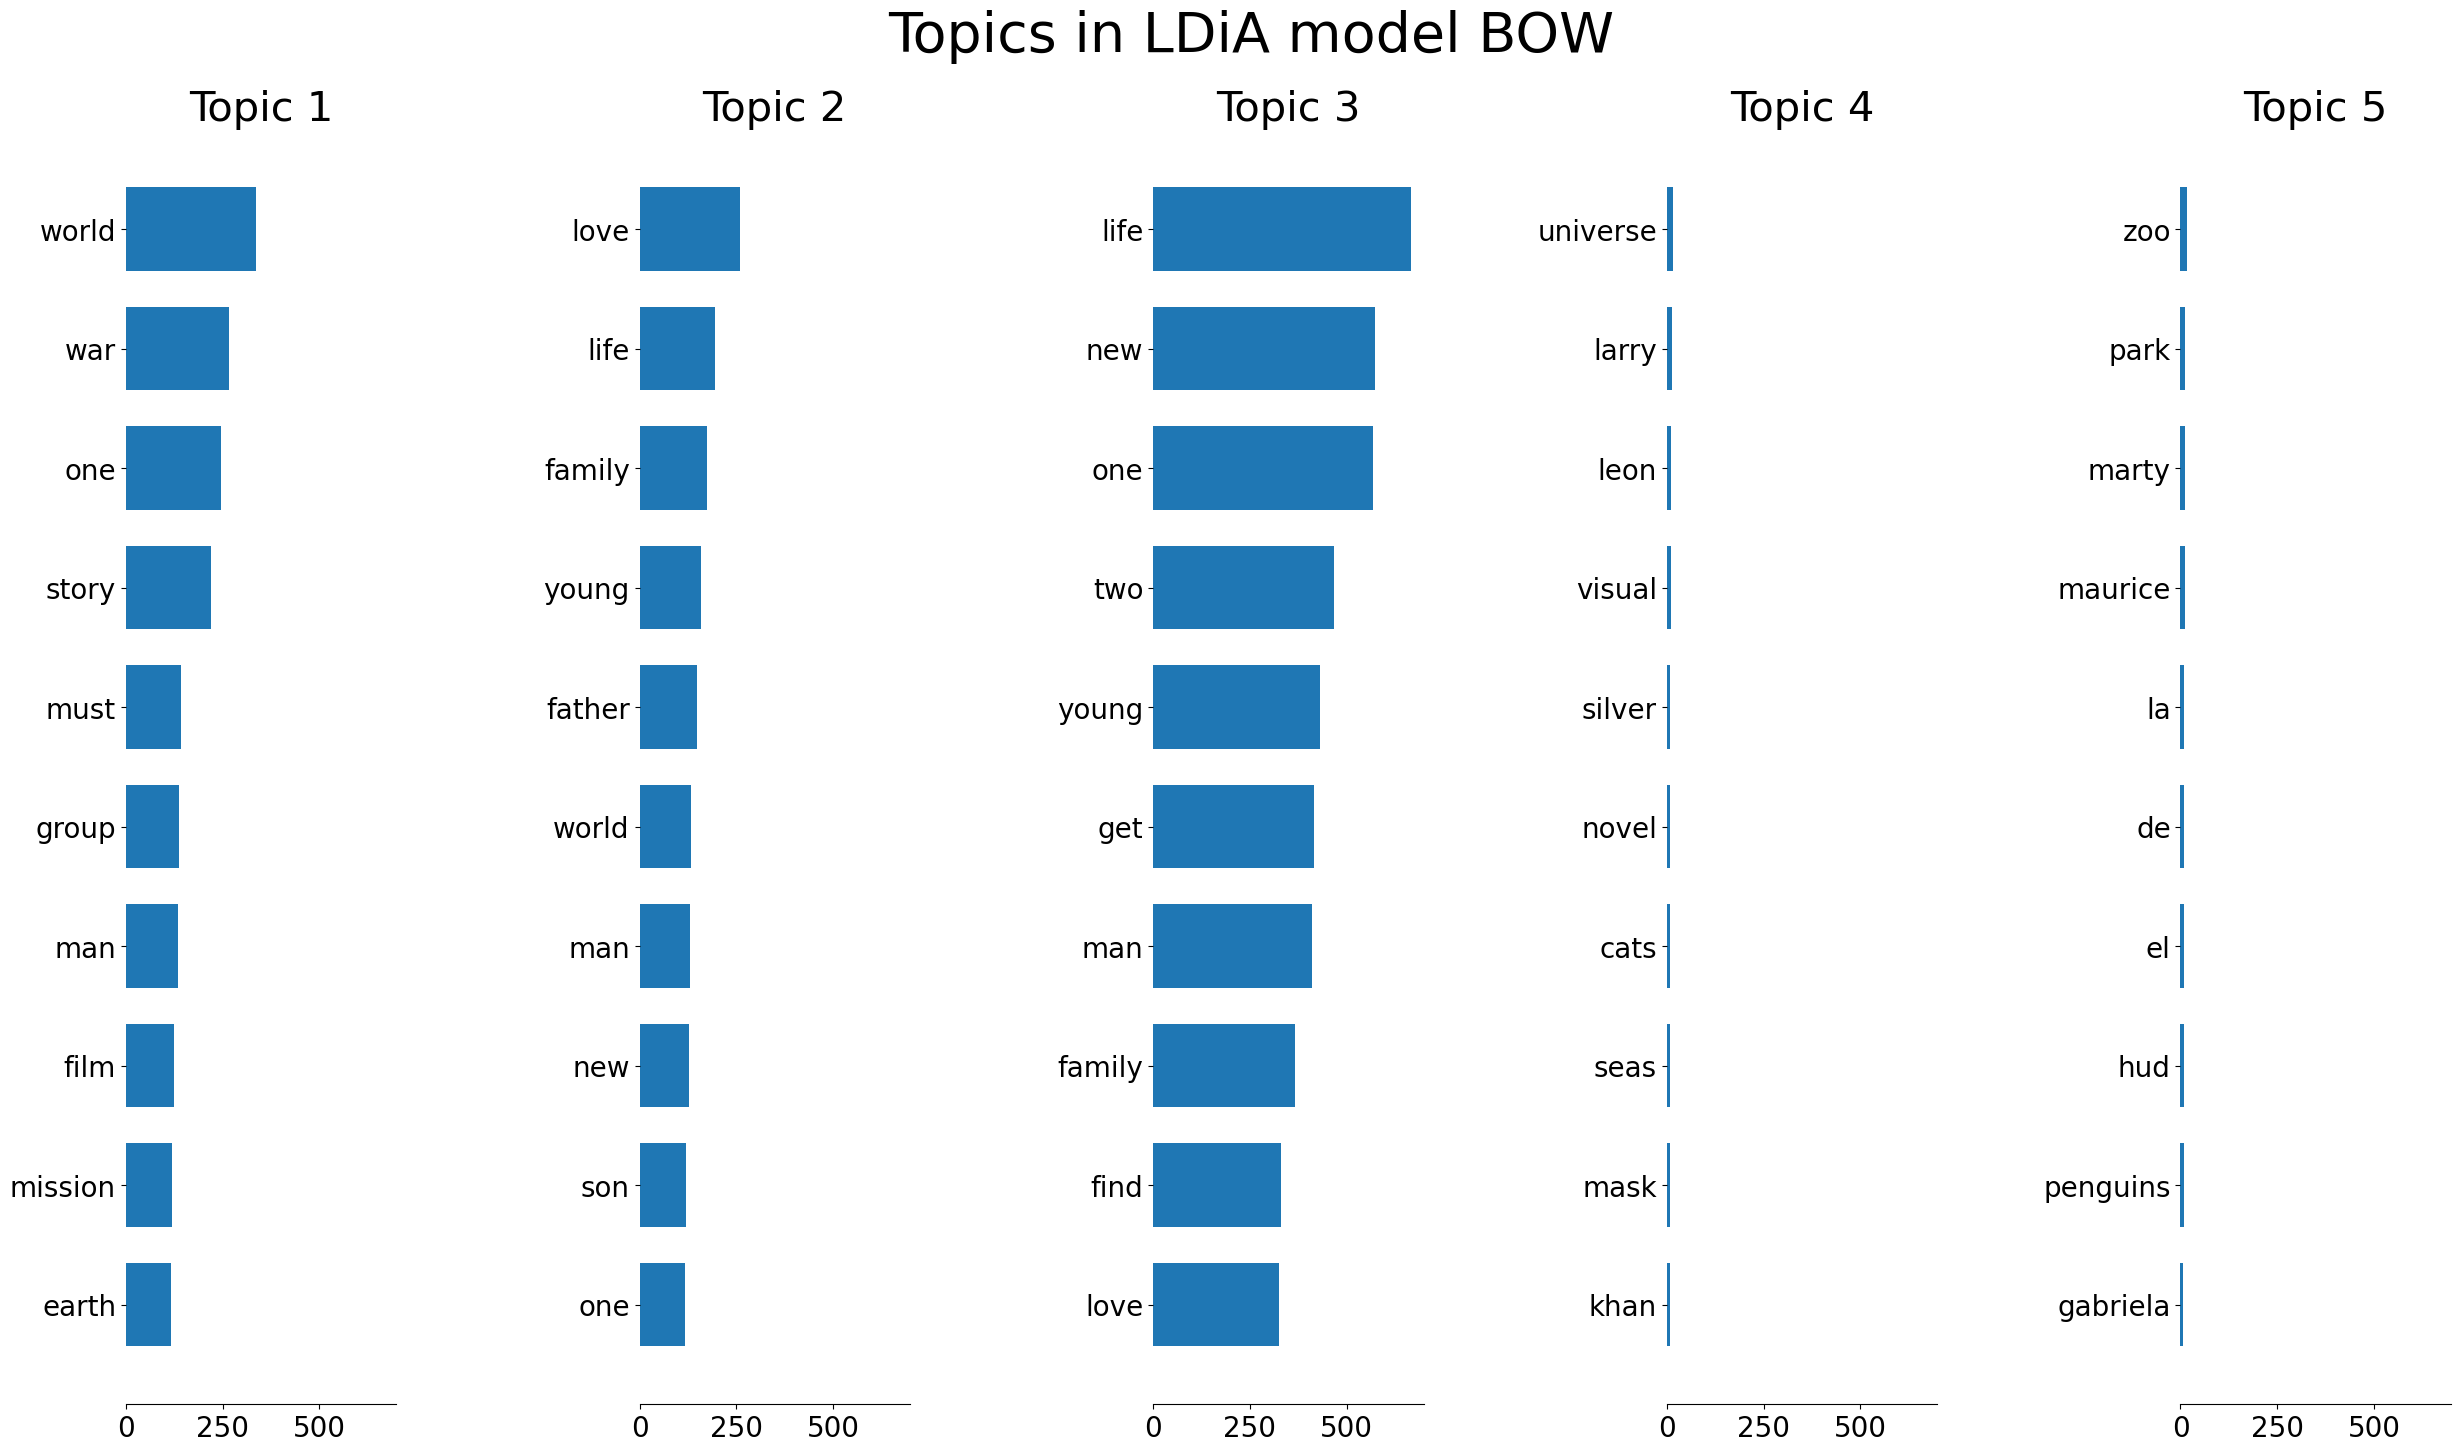
\includegraphics[scale=.1]{img/nlp2.png}

{\small
  Figure 14: Topics in LDiA model BOW
  \par
  \vspace{6pt}
}

In our exploration, we visually represented the topics using both Bag of Words (BOW) and Term Frequency-Inverse Document Frequency (TFIDF) methods. To our surprise, the visualizations of the topic modeling using these methods were strikingly similar. Typically, BOW highlights the raw frequencies of terms, sometimes losing some nuance, while TFIDF emphasizes terms more uniquely important to the document in the context of the larger corpus. In this case, both approaches revealed a similar set of terms with similar frequencies for each topic, such as 'one,' 'new,' 'man,' and 'world.' This unusual similarity indicates that the weighting mechanism TFIDF uses was not significant enough to provide any preeminence of specific terms that dominate the topic regardless of the weighting scheme.

\subsubsection{Feature Extraction}

The Natural Language Processing (NLP) task advanced significantly following the text processing phase, entering the critical stage of feature extraction. Here, the strategic implementation of Term Frequency (TF) and Term Frequency-Inverse Document Frequency (TF-IDF) techniques played a pivotal role. These methods were instrumental in extracting relevant features from the text, enabling a deeper and more precise exploration of the processed data. The application of these feature extraction techniques was crucial in identifying significant patterns and trends within the dataset, highlighting the subtle intricacies and complexities of textual data.
\par
\vspace{6pt}


\includegraphics[scale=.7]{img/nlp3.png}

{\small
  Figure 15: Word Cloud
  \par
  \vspace{6pt}
}

In the word cloud above we see results of extracting relevant features from the text. We see that the more a word is used in the text description, the larger it is displayed on the word cloud. This highlights the frequent use of words that are central to the overall message or theme of the text. By identifying and analyzing these frequently used words, we can gain valuable insights into the core concepts and topics being discussed.

\subsubsection{Searching for Similar Movies}

Building on this foundation, the NLP's prowess was further exemplified in the task of searching for similar movies. This application showcased the remarkable strength of NLP in forging meaningful connections between diverse texts. The employed algorithm displayed a notable proficiency in identifying and matching similar themes across a range of movie descriptions, demonstrating the advanced capabilities of NLP in thematic matching and content analysis. The success in this particular task underscored the effectiveness of the preceding feature extraction phase, as the accurate identification of themes and patterns in text is contingent upon the quality of the extracted features. This synergy between feature extraction and thematic analysis highlights the cohesive and comprehensive nature of the NLP process, underlining its importance in extracting valuable insights from complex textual datasets. 

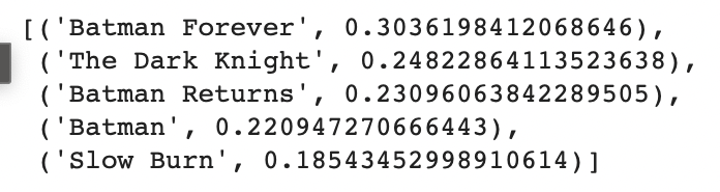
\includegraphics[scale=.5]{img/nlp4.png}

{\small
  Figure 16: Similar movies to “The Dark Knight Rises”
  \par
  \vspace{6pt}
}

If I am assuming that I like “The Dark Knight Rises”, It would recommend these movies, because we used the cosine similarity metric to measure the similarity so the algorithm can suggest movies based on their descriptions in the dataset. 

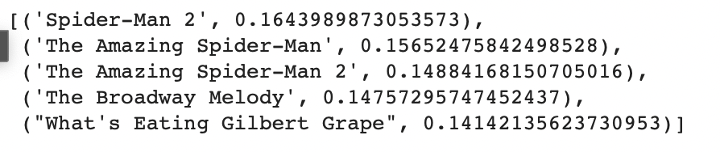
\includegraphics[scale=.5]{img/nlp5.png}

{\small
  Figure 17: Similar movies to “Spider-man 3”
  \par
  \vspace{6pt}
}

By analysing the top recommended movies for “Spider-man 3”, there appears to be a mix of genres, indicating that the recommendation system considers various aspects of movie descriptions.

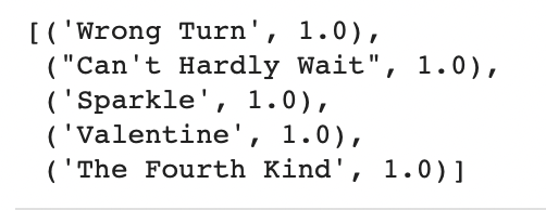
\includegraphics[scale=.5]{img/nlp6.png}

{\small
  Figure 18: Opposite movie recommendations to “Harry Potter and the Half-Blood Prince”
  \par
  \vspace{6pt}
}

If you were to hate the movie “Harry Potter and the Half-Blood Prince”, we could use the opposite cosine similarity metrices to find the opposite movie. This would come as the recommended movies. 

\section{Conclusion}

In conclusion this research has delved into machine learning (ML) and natural language processing (NLP) revealing innovative ways to apply these technologies in tasks such as classification, clustering, regression and textual analysis. By examining datasets related to health monitoring, urban mobility and housing this study has showcased the versatility and effectiveness of ML and NLP techniques. The collaboration between these two fields has provided us with an understanding of datasets opening the doors for future collaborations across different domains. This research highlights how combining ML and NLP can unearth insights that serve as a foundation for making informed decisions, in various applications.

\end{multicols}

% Bibliography
\bibliographystyle{agsm}
\bibliography{sample}


\phantom{
  \cite{lane_natural_2019}
  \cite{kononenko_machine_2007}
  \cite{noauthor_sklearnneighborskneighborsregressor_nodate}
  \cite{ali_data_2014}
  \cite{shen_influence_2021}
  \cite{sen_supervised_2020}
  \cite{madhulatha_overview_2012}
  \cite{gulli_deep_2017}
}


% End the two-column layout
\end{document}
